\chapter{Evaluation}
\label{chapter:evaluation}

Before we evaluate the system, we will make a few notes that apply to the evaluation of the system as a whole.

\section{Notes}

All the tests and benchmarks were performed on a single machine.
The machine has 16GB of RAM, an M1 Apple Silicon processor 3200 MHz, and a 512GB SSD.
Due to these specs, the benchmarks are run with files between 1MB and 100MB.
We ran benchmarks with files up to 1GB and the results were consistent with the results from the smaller files,
i.e., the algorithms exhibit the same behavior, but rerunning the benchmarks takes a lot of time.

The system is written in Rust, which means no garbage collection or runtime overhead,
which we can see from running 1000 instances in \autoref{fig:1000-instances}.
Because the system consumes almost no resources when idle,
we can run many instances on a single machine.
We will not account for the overhead of the system being idle in the benchmarks.

\begin{figure}
    \centering
    \includegraphics[width=350pt]{gfx/1000-instances.png}
    \captionof{figure}{Starting 1000 instances}
    \label{fig:1000-instances}
\end{figure}

\section{Performance of the system}

Our final goal is to augment a distributed storage system with verification based on PoR.
In the process we want to ensure that the performance of the system is not degraded.
The main part we are changing is the way files are stored, by injecting the PoR initialization,
and the idle state of the peers --- during which they perform audits.
We performed the benchmarks starting with 10 and up to 100 peers in the network.
Since the tests are run on a single machine, running more peers would not give us any useful information,
because the resources of the machine will be exhausted from running the peers in idle state.
This is also the reason we are using files of size up to 10MB.
Larger files would take more time to read and write to disk,
but would not give us any additional information about the performance of the system.
The results of the benchmarks are shown in \autoref{table:storage_vs_kad} \autoref{table:storage_times}.

From \autoref{table:storage_vs_kad} we can see the overhead of running the PoR algorithm and
writing the metadata to the ledger.
It starts becoming noticeable for files larger than 1MB, where it takes six to ten times longer
to store the file.
This overhead is expected, as we are running the PoR algorithm for each peer that stores the file,
and we write the metadata to the ledger.
It is also not a problem because it is a one-time operation.

Let us look at the Time without Verifier first.
In these tests the first node that the storage request is sent to is not running the Verifier.
Files under 100 KB have almost no impact on the system's performance.
Saving 1 MB takes around 270 ms, which we can conclude by taking the 320 ms, which is the total
time for the request, and subtracting the 50 ms that each request takes to be processed.
This tendency is also visible for the 10 MB files, which take 2700 ms, which is 270 ms per 1 MB
(we are ignoring the 50 ms processing time, as it becomes negligible for larger files).

It is interesting to note that having 10 or 100 nodes in the network does not seem to impact the
time to store files.
This is the case because before running each benchmark we wait for the peers in the network
to connect to each other.
We do not run the tests immediately after a cold start of the system.

Next, we look at the Time with Verifier running.
The times to process a request here are significantly higher.
This is mainly due to the outlier requests, which have to be processed while a verification is running.
With our current architecture, the ledger module and the Kademlia swarm module are both singleton modules,
locked behind mutexes, to ensure that no race conditions occur.
This causes the Verifier to occasionally take a hold of these mutexes and block the
storage requests from being processed.
This can be circumvented by running a pool of connections to the ledger and the swarm.
We have left this for future work as it can be circumvented by each peer running 2 nodes ---
one for storage and one for verification.

\begin{landscape}
  \begin{table}[h]
    \centering
    \myfloatalign
    \pgfplotstabletypeset[
    every head row/.style={ before row=\toprule, after row=\midrule },
    every last row/.style={ after row=\bottomrule },
    columns={npeers, data, kad, time, timever, p99},
    columns/npeers/.style={string type, column name=\shortstack{\textsc{Number} \\ \textsc{of peers}}, dec sep align, fixed, fixed zerofill },
    columns/data/.style={ column name=\shortstack{\textsc{Data} \\ \textsc{stored}}, column type=r, string type},
    columns/kad/.style={ column name=\shortstack{\textsc{Without PoR}}, string type, column type=r},
    columns/time/.style={ column name=\shortstack{\textsc{Time without} \\ \textsc{Verifier running}}, string type, column type={r}},
    columns/timever/.style={ column name=\shortstack{\textsc{Time with} \\ \textsc{Verifier running}}, string type, column type=r},
    columns/p99/.style={ column name=\shortstack{\textsc{Longest} \\ \textsc{request time}}, string type, column type=r},
    ]{./data/store.csv}
    \caption{Storing files in the system with replication factor of 3}
    \label{table:storage_vs_kad}
  \end{table}
\end{landscape}

\begin{table}
  \myfloatalign
  \pgfplotstabletypeset[
  every head row/.style={ before row=\toprule, after row=\midrule },
  every last row/.style={ after row=\bottomrule },
  columns={npeers, data, time, timever, p99},
  columns/npeers/.style={string type, column name=\shortstack{\textsc{Number} \\ \textsc{of peers}}, dec sep align, fixed, fixed zerofill },
  columns/data/.style={ column name=\shortstack{\textsc{Data} \\ \textsc{stored}}, column type=r, string type},
  columns/time/.style={ column name=\shortstack{\textsc{Time without} \\ \textsc{Verifier running}}, string type, column type={r}},
  columns/timever/.style={ column name=\shortstack{\textsc{Time with} \\ \textsc{Verifier running}}, string type, column type=r},
  columns/p99/.style={ column name=\shortstack{\textsc{Longest} \\ \textsc{request time}}, string type, column type=r},
  ]{./data/store.csv}
  \caption{Storing files in the system with replication factor of 3}
  \label{table:storage_times}
\end{table}

\section{Proof of Retrievability (PoR)}
\label{section:por-evaluation}

In this section, we will evaluate how the PoR system performs in a real-world scenario.
We have discussed how PoR is used to ensure the integrity of the data stored on the nodes.
Now, we will evaluate how viable is it to use PoR in the system.
Does it adhere to the \autoref{section:requirements}?
And is it fast enough to be used in a real-world scenario?

\subsection{How many audits can we perform in parallel?}

The audit is a two-step process.
First, the Verifier sends the challenge to the Keeper and then the Keeper responds with the proof.

We expect the load on the Verifier to be negligible, while the load on the Keeper to be significant.
The Verifier should do as little work as possible,
because we want to perform as many audits as possible in parallel.
This way we can ensure that audits are performed often enough to ensure the integrity of the data.
The load on the Keeper is expected to be high,
because the Keeper needs to read the file from disk and execute the PoR algorithm.
Ideally that algorithm will be linear in time complexity in the size of the file.

The Verifier performs 2 operations --- sending the challenge and verifying the proof.
We benchmarked these operations and the results are shown in \autoref{fig:por-verifier-create-challenge}
and \autoref{fig:por-verifier-audit-challenge}.

The results show that generating the challenge and auditing are both very fast operations ---
for a 100MB file, the Verifier can generate the challenge in 0.027ms and
audit the proof in 0.137ms.

We can observe something interesting the in the results ---
the graph looks almost logarithmic, instead of linear.
This is due to cache locality since both the operations are executing code on sequential memory addresses.
Both the challenge and the response are essentially a vector of numbers,
which is a very cache-friendly data structure.

\begin{figure}
  \myfloatalign
  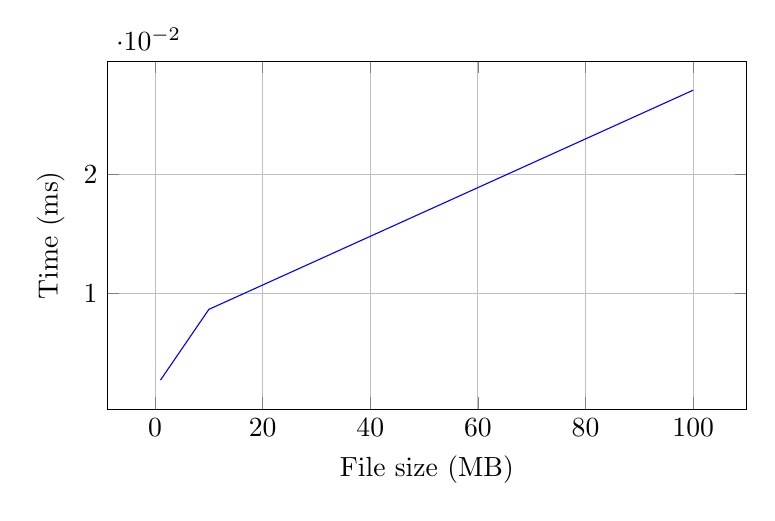
\begin{tikzpicture}
    \begin{axis}[
      xlabel={File size (MB)},
      ylabel={Time (ms)},
      grid=major,
      width=0.8\textwidth,
      height=6cm,
    ]
    \addplot[mark=., blue] coordinates {
      (1, 0.002736)
      (10, 0.008674)
      (100, 0.027069)
    };
    \end{axis}
  \end{tikzpicture}
  \caption{Time required for the Verifier to create the challenge for PoR.}
  \label{fig:por-verifier-create-challenge}
\end{figure}

\begin{figure}
  \myfloatalign
  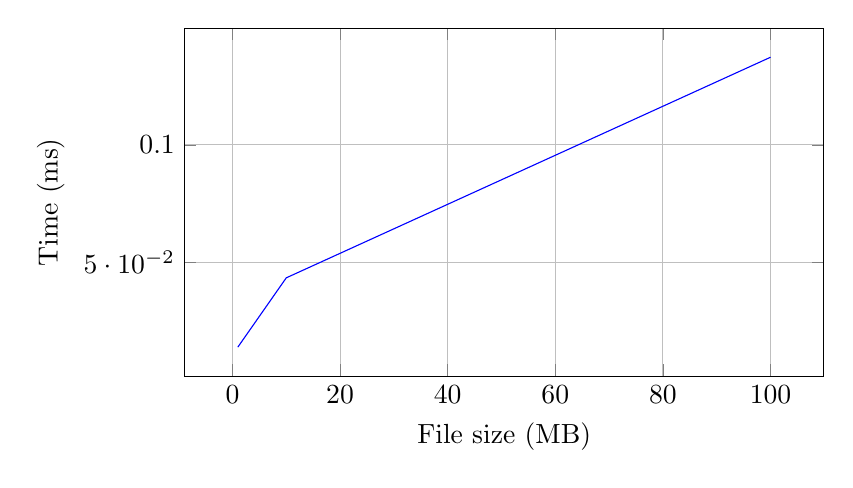
\begin{tikzpicture}
    \begin{axis}[
      xlabel={File size (MB)},
      ylabel={Time (ms)},
      grid=major,
      width=0.8\textwidth,
      height=6cm,
    ]
    \addplot[mark=., blue] coordinates {
      (1, 0.013733)
      (10, 0.043281)
      (100, 0.137354)
    };
    \end{axis}
  \end{tikzpicture}
  \caption{Time required for the Verifier to audit the challenge response PoR.}
  \label{fig:por-verifier-audit-challenge}
\end{figure}

The Keeper performs 1 operation --- generating the proof.
This is done by reading the file from disk and running the PoR algorithm on it.
The PoR algorithm is expected to be linear in time complexity in the size of the file.
We benchmarked this operation and the results are shown in \autoref{fig:por-keeper-challenge-generate}.

The operation gets slower as the file size increases.
In theory the time complexity should be linear, but it is superlinear in practice.
This is most likely caused by the unoptimized matrix multiplication algorithm that we are using to
implement PoR.

\begin{figure}
  \myfloatalign
  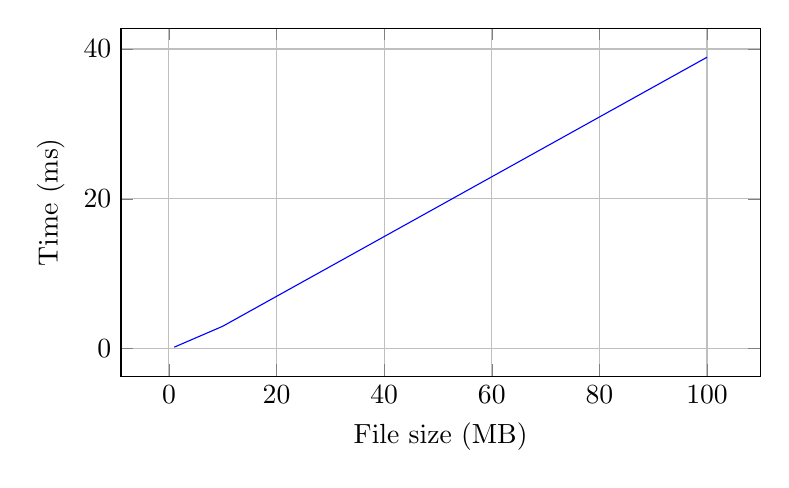
\begin{tikzpicture}
    \begin{axis}[
      xlabel={File size (MB)},
      ylabel={Time (ms)},
      grid=major,
      width=0.8\textwidth,
      height=6cm,
    ]
    \addplot[mark=., blue] coordinates {
      (1, 0.21614)
      (10, 3.002728)
      (100, 38.900041)
    };
    \end{axis}
  \end{tikzpicture}
  \caption{Time required to create the challenge response (proof) for PoR on the Keeper side, without reading the file from disk.}
  \label{fig:por-keeper-challenge-generate}
\end{figure}

\subsection{Is PoR the limiting factor in the system?}

One of the main questions we want to answer in this thesis is whether the validation component
affects the system's performance.
From the results we can see that while the evaluation aspect introduces more workload,
however, it is within reasonable levels.

In the previous section we saw that the Verifier can generate the challenge and audit the proof very quickly.
Since the speed of reading from an SSD is on average 7000 MB/s, the PoR protocol in the Verifier
will not affect the system's performance.
It is more likely, that the network connection between the Verifier and the Ledger will be the limiting factor,
but we will not evaluate network speeds as they are out of the scope of this thesis.

The Keeper can generate the proof at a rate of 38ms for a 100 MB.
This is faster than the access speed of an HDD, which is around 500 MB/s or 200ms for a 100 MB.
However, it is slower than the access speed of an SSD, which is around 7000 MB/s or 14ms for a 100 MB.
Whether the PoR protocol is the limiting factor or not depends on what kind of storage the Keeper is using.

In conclusion, the Verifier can send challenges in parallel, but the Keeper nodes will still be
the limiting factor in the system.

\section{How fast are malicious behaviors detected?}

All files are verified each cycle.
The Verifiers split the work of verifying the files based on the file's key.
As an example, if we have two peers (2 Keepers and 2 Verifiers),
the Verifiers would split the files of each Keeper and take turns verifying them
during alternating cycles.
This is illustrated in \autoref{fig:2-verifiers}.

\begin{figure}
    \centering
    \includegraphics[width=350pt]{gfx/2-verifiers.png}
    \captionof{figure}{Splitting the ID space between two Verifiers}
    \label{fig:2-verifiers}
\end{figure}

This means that when a peer becomes malicious they have at most one cycle of time,
before they are detected.
We are running the benchmarks in \autoref{table:verify_detection_times} with various amount of data in the system.
The cycle times are chosen arbitrarily in order to provide an overview of how the system behaves with
different cycle times and to show the connection between the amount of data and the cycle length.
The cycle time when running the system in production should be set to a value proportional to
the amount of data and number of files stored in the network.
We are running the benchmarks with 1 corrupt peer in the network,
because if we have more the chance of a corrupt peer being detected increases.
We are interested in how long it takes to discover the first signs of misbehaving in the network.
The general observation, which is not surprising, is that the more files we have in the network,
the faster it is to discover a corrupt peer,
because the greater the chance it is for the corrupt peer to store a file.
For example, with 100 peers and 100 files in the system, the corrupt peer is expected to store 1 file,
That means that all the files need to be verified in order to discover the corrupt peer.
This is even more apparent with 10 peers where the time to discover a corrupt peer with 1000 files is
41ms in comparison with 1120ms for 100 files.

\begin{table}
  \myfloatalign
  \pgfplotstabletypeset[
  every head row/.style={ before row=\toprule, after row=\midrule },
  every last row/.style={ after row=\bottomrule },
  columns={npeers, data, cycle_time, time},
  columns/npeers/.style={string type, column name=\shortstack{\textsc{Number} \\ \textsc{of peers}}, dec sep align, fixed, fixed zerofill },
  columns/data/.style={ column name=\shortstack{\textsc{Data} \\ \textsc{stored}}, column type=r, string type},
  columns/cycle_time/.style={ column name=\shortstack{\textsc{Time per} \\ \textsc{cycle}}, string type, column type={r}},
  columns/time/.style={ column name=\shortstack{\textsc{Time to discover} \\ \textsc{corrupt peer}}, string type, column type=r},
  ]{./data/verify.csv}
  \caption{Time to discover a corrupt peer in the network with 1 corrupt peer}
  \label{table:verify_detection_times}
\end{table}

\section{Reputation system based on a ledger}

The results of the PoR are stored in a ledger, which acts as the source of truth for
the performance of the peers in the network.
While ideally we would like to have a decentralized ledger, for the sake of simplicity
we will use a centralized ledger in our evaluation.
For the purposes of evaluation we could have used a simple SQL database or a local file,
however, we used Immudb because it is what we used in the previous iterations of the system
and at the time we were exploring it as a potential solution for the ledger.

\subsection{Immudb performance}

Having a centralized ledger means we have a potential bottleneck.
The benchmarks that the authors of Immudb are presented in \autoref{tab:immudb}.
While processing more than a million requests per second is impressive,
it is not performance we can expect because we are storing the metadata for PoR in the ledger,
which is considerably more than empty requests.
Based on the benchmarks we can conclude that we can use Immudb as a ledger and have
a throughput of more than a million requests per second,
but we need a distributed version of Immudb,
because the limiting factor becomes the network throughput and the disk read/write speed.
Immudb is not bad as a ledger, but the fact it is not distributed limits its use in a production system.

\begin{table}
  \myfloatalign
  \pgfplotstabletypeset[
    every head row/.style={ before row=\toprule, after row=\midrule },
    every last row/.style={ after row=\bottomrule },
    columns={entries, workers, batch, batches, time, entries_per_s},
    columns/entries/.style={string type, column name=\shortstack{\textsc{Entries}}, column type={r}},
    columns/workers/.style={column name=\shortstack{\textsc{Workers}}, column type={r}},
    columns/batch/.style={column name=\shortstack{\textsc{Batch}}, column type={r}},
    columns/batches/.style={column name=\shortstack{\textsc{Batches}}, column type={r}},
    columns/time/.style={column name=\shortstack{\textsc{Time (s)}}, column type={r}},
    columns/entries_per_s/.style={string type, column name=\shortstack{\textsc{Entries/s}}, column type={r}},
  ]{./data/immudb.csv}
  \caption{Immudb performance according to the authors \cite{immudb-gh}}
  \label{tab:immudb}
\end{table} 

\subsection{What makes a ledger a good choice for the reputation system?}

% \wtf{TODO: I'm still playing around with this idea, I'm not sure if this is the best way to do it.
% Perhaps the staked reputation will be returned gradually with each successful audit.
% The whole idea of adding "staking" is to ensure the peer has a big hit in reputation from the beginning.
% This way a new peer in the network cannot just accept a lot of files as soon as it joins and then go offline.}
% Every time an audit is performed the reputation of the peer on which the audit was performed is adjusted.
% If the audit is successful, the reputation of the peer is increased,
% and if the audit fails, the reputation of the peer is decreased.
% Finally, a peer is awarded reputation points for performing audits.
% The increase and decrease numbers are configurable and can be adjusted to fit the network requirements.
% We will discuss the different possibilities for adjusting the reputation in the \autoref{chapter:evaluation}
\wtf{Answer the question from the hypothesis: 
    Is a reputation system based on a ledger a viable measure against malicious nodes?
}
\wtf{
    I think in this section I'll cover what are a ledger's strong points and guarantees that
    would be beneficial for the reputation system.
}

% We need to evaluate the proper penalties and rewards for the nodes.
% A good balance is needed between rewards and penalties to ensure that a node is
% going to perform enough work for the system before being able to harm it.
% Part of this evaluation will be:
% \begin{enumerate}
%     \item How much reputation points a node stakes when it stores a file?
%     \item How much reputation points a node loses when it fails an audit?
%     \item How much reputation points a node gains when it performs an audit?
%     \item How much reputation points a node loses when it's discovered to not be performing audits?
%     \item What is the starting reputation for new nodes?
%     \item How do nodes increase their reputation at the very beginning?
%     \item Does having high reputation give the node any benefits?
% \end{enumerate}

% Nodes with very high reputation could easily become malicious as they can absorb the penalties.
% We need to solve this problem by either having a maximum reputation or by having the penalties be
% percentage-based.

% We need to answer the question of how often audits should be performed and how often nodes should
% check the audit results of others.
% The overhead of performing audits should be as low as possible, but the audits should be performed often enough
% to ensure the integrity of the data.

% Finding the balance between audits and the overhead of the audits, and the penalties and rewards for the nodes
% is crucial for the success of the system.
% We will evaluate the system by running it with different parameters and observing the behavior of the nodes.
% We will discuss the details and the results of the evaluation in \ref{chapter:evaluation}.

\section{Balancing the reputation system}

\wtf{for each 100k files added to the system, we need to increase the cycle time by...,
for each 1GB of data stored in the system, we need to increase the cycle time by...,
for each X number of peers in the network, we need to increase the cycle time by...}

\subsection{Gaining and losing reputation as a Keeper}
\wtf{Cover how the reputation awards should be balanced against the punishments to ensure
that the system can maintain its integrity. We will assume that a node dropping to negative reputation
results in it being kicked out of the network.}

\subsection{Gaining and losing reputation as a Verifier}

\wtf{Do the same for checking the previous Verifier's audit as we do for the Keeper}
\wtf{ give peers some leeway from being offline - give it some time to be offline before punishing.  }


\section{Using Rust}

\wtf{TODO: MOVE THIS TO THE END}

\wtf{Cover what are the strong/weak points of using Rust for such a system.}

\section{Summary}
% at the end of the evaluation add a sumamry - is the system viable or should you use amazon,
% is the system recommened for production for companies - for what use cases is it recommened,
% basically add stuff something akin to a conclusion that then can be used in the conclusion chapter,
% eval - if someone sees this PoR for the first time - how expensive is it, what is the overhead, why not use
% amazon/other s3
% por could be good for when we store files in s3 and we use por to check the integrity of the files
